\begin{figure}[H]
    \centering
    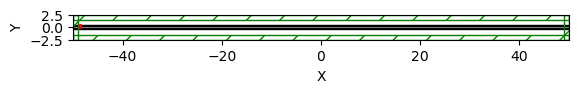
\includegraphics[width=0.8\linewidth]{Figures/wg_design.png}
    \caption{}
    \label{fig:wg_design}
\end{figure}

\begin{figure}[H]
    \centering
    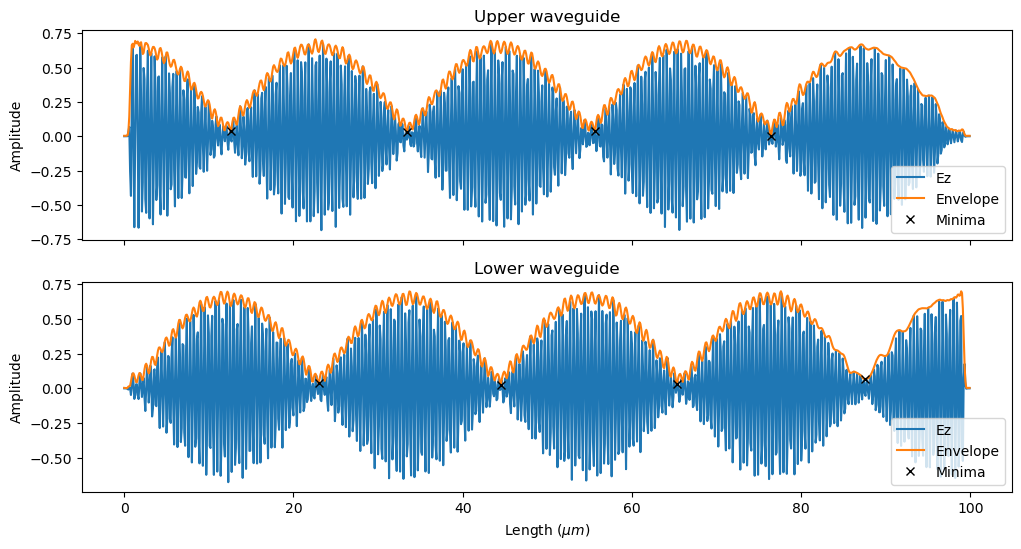
\includegraphics[width=0.8\linewidth]{Figures/wg_field.png}
    \caption{}
    \label{fig:wg_field}
\end{figure}

\begin{figure}[H]
    \centering
    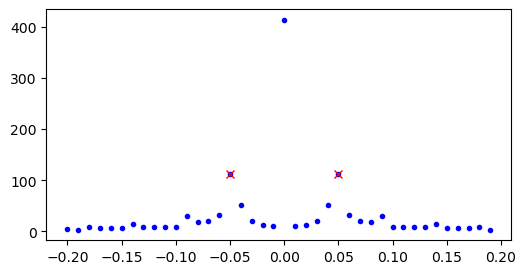
\includegraphics[width=0.5\linewidth]{Figures/wg_fft.png}
    \caption{}
    \label{fig:wg_fft}
\end{figure}

\begin{figure}[H]
    \centering
    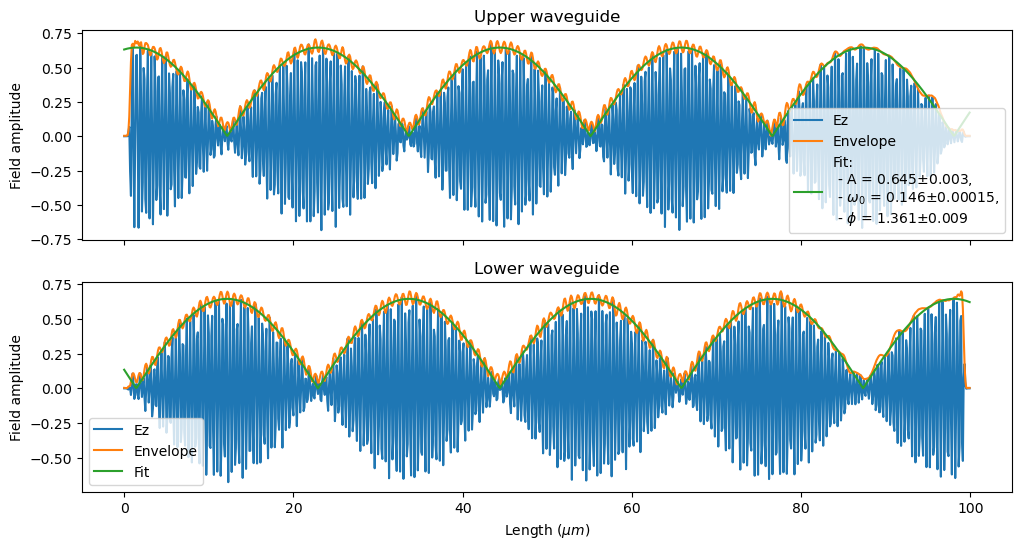
\includegraphics[width=0.8\linewidth]{Figures/wg_field_fit.png}
    \caption{}
    \label{fig:wg_field_fit}
\end{figure}

\begin{figure}[H]
    \centering
    \begin{subfigure}[b]{0.45\linewidth}
        \centering
        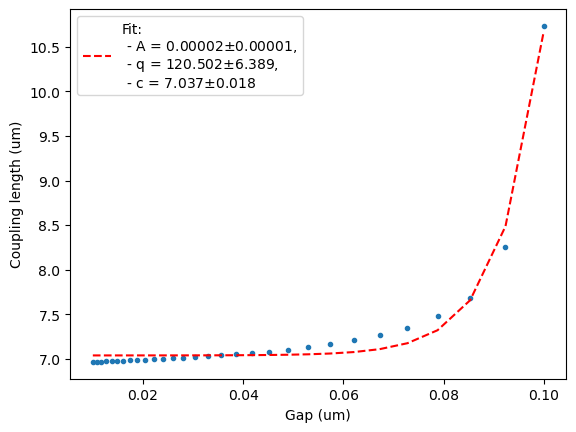
\includegraphics[width=\linewidth]{Figures/wg_coupling_vs_gap.png}
        \caption{}
        \label{fig:wg_coupling_vs_gap}
    \end{subfigure}
    \hfill
    \begin{subfigure}[b]{0.45\linewidth}
        \centering
        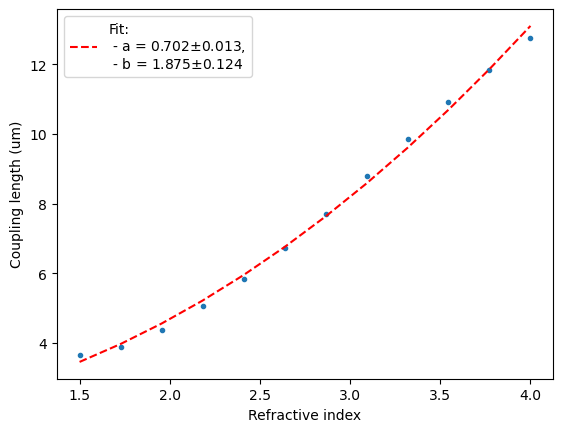
\includegraphics[width=\linewidth]{Figures/wg_coupling_vs_index.png}
        \caption{}
        \label{fig:wg_coupling_vs_index}
    \end{subfigure}
\end{figure}

\begin{figure}[H]
    \centering
    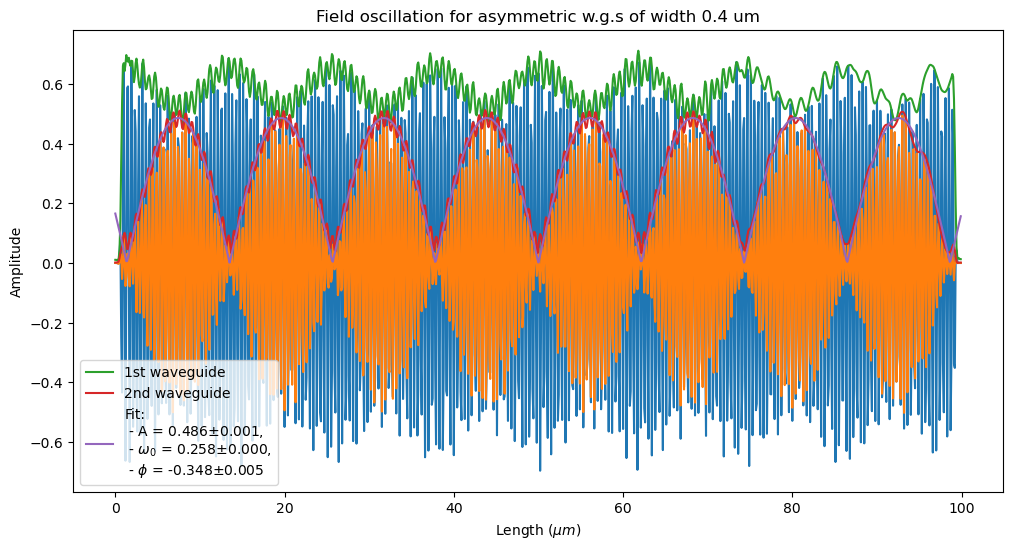
\includegraphics[width=0.8\linewidth]{Figures/wg_field_asymm.png}
    \caption{}
    \label{fig:wg_field_asymm}
\end{figure}

\begin{figure}[H]
    \centering
    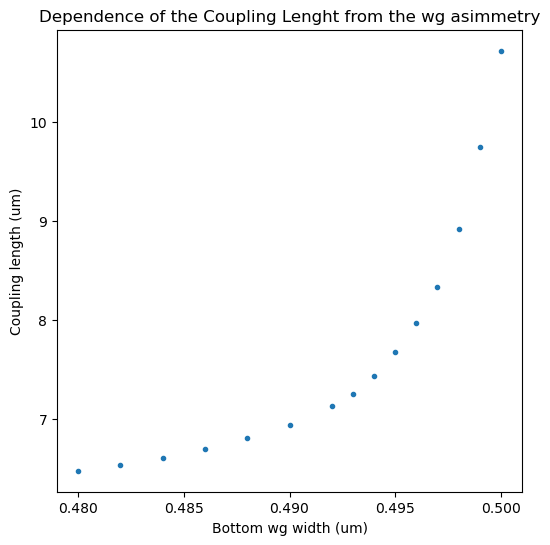
\includegraphics[width=0.6\linewidth]{Figures/wg_coupling_vs_asymm.png}
    \caption{}
    \label{fig:wg_coupling_vs_asymm}
\end{figure}